
It the previous chapter the proposed load balancer is verified to be portable, redundant and scalable in 1Gbps network.
It is also important to investigate its validitys in 10Gbps network.
In this chapter the performance level of the proposed load balancer is evaluated.
The author carries out throughput measurements of ipvs, ipvs-tun, and iptables DNAT in 10Gbps environment.
The author clarifies the reasons for performance limitations and discusses improvement.
The author also proposes a novel software load balancer using eXpress Data Plane(XDP) technology and presents preliminary experimental results.

\section{Throughput measurement in 10G network}

In order to evaluate the performance levels of the proposed load balancer in a 10Gbps network environment, the author carried out throughput measurements.
Table~\ref{tab:hw_sw_spec_10g} summarizes the hardware and software specification used in the experiment.
Bare metal servers with Intel X550 network card was used.
The X550 NIC has a maximum of 64 rx-queues, and 16 of them are activated by the driver at the boot time since there are 16 logical CPUs.
The setting \enquote{(RSS, RPS)=(on, off)} is used because interrupts from each of 16 rx-queues can be assigned to separate logical cores.
And hence, packet processing is distributed to all of the 16 logical cores, which results in the best performance in most of the cases.
The host-gw mode is used as the backend mode of the flannel overlay network.

{
\setlength{\tabcolsep}{1em}
\renewcommand{\arraystretch}{1.2}

\begin{table}[h]
  \centering
  \begin{tabular}{ll}
    \hline 
    \multicolumn{2}{l}{[Hardware Specification]}   \\
    & CPU: Xeon E5-2450 2.10GHz x 8 (with Hyper Threading) \\
    & Memory: 32GB \\
    & NIC: Intel X550 with 64 rx-queues (16 activated), 10 Gbps \\
    & (Node x 6, Load Balancer x 1, Client x 1)) \\
    & \\
    \multicolumn{2}{l}{[Node Software]}  \\
    & OS: Debian 9.5, linux-4.16.8 \\
    & Kubernetes v1.5.2 \\
    & flannel v0.7.0 \\
    & etcd version: 3.0.15 \\
    & \\
    \multicolumn{2}{l}{[Container Software]}   \\
    & Keepalived: v1.3.2 (12/03,2016) \\
    & nginx : 1.15.4(web server) \\
  \hline 
  \end{tabular}
  \par\bigskip
  \centering
  \begin{minipage}{0.9\columnwidth}
    \caption[Hardware and software specifications for 10Gbps experiment]{
      Hardware and software specifications for 10Gbps experiment.
      There are 16 rx-queues activated for the NIC, to match the number of logical CPUs.
    }
    \label{tab:hw_sw_spec_10g}
  \end{minipage}
\end{table}
}

\begin{figure}[h]
  \begin{subfigure}[t]{\columnwidth}
    \centering
    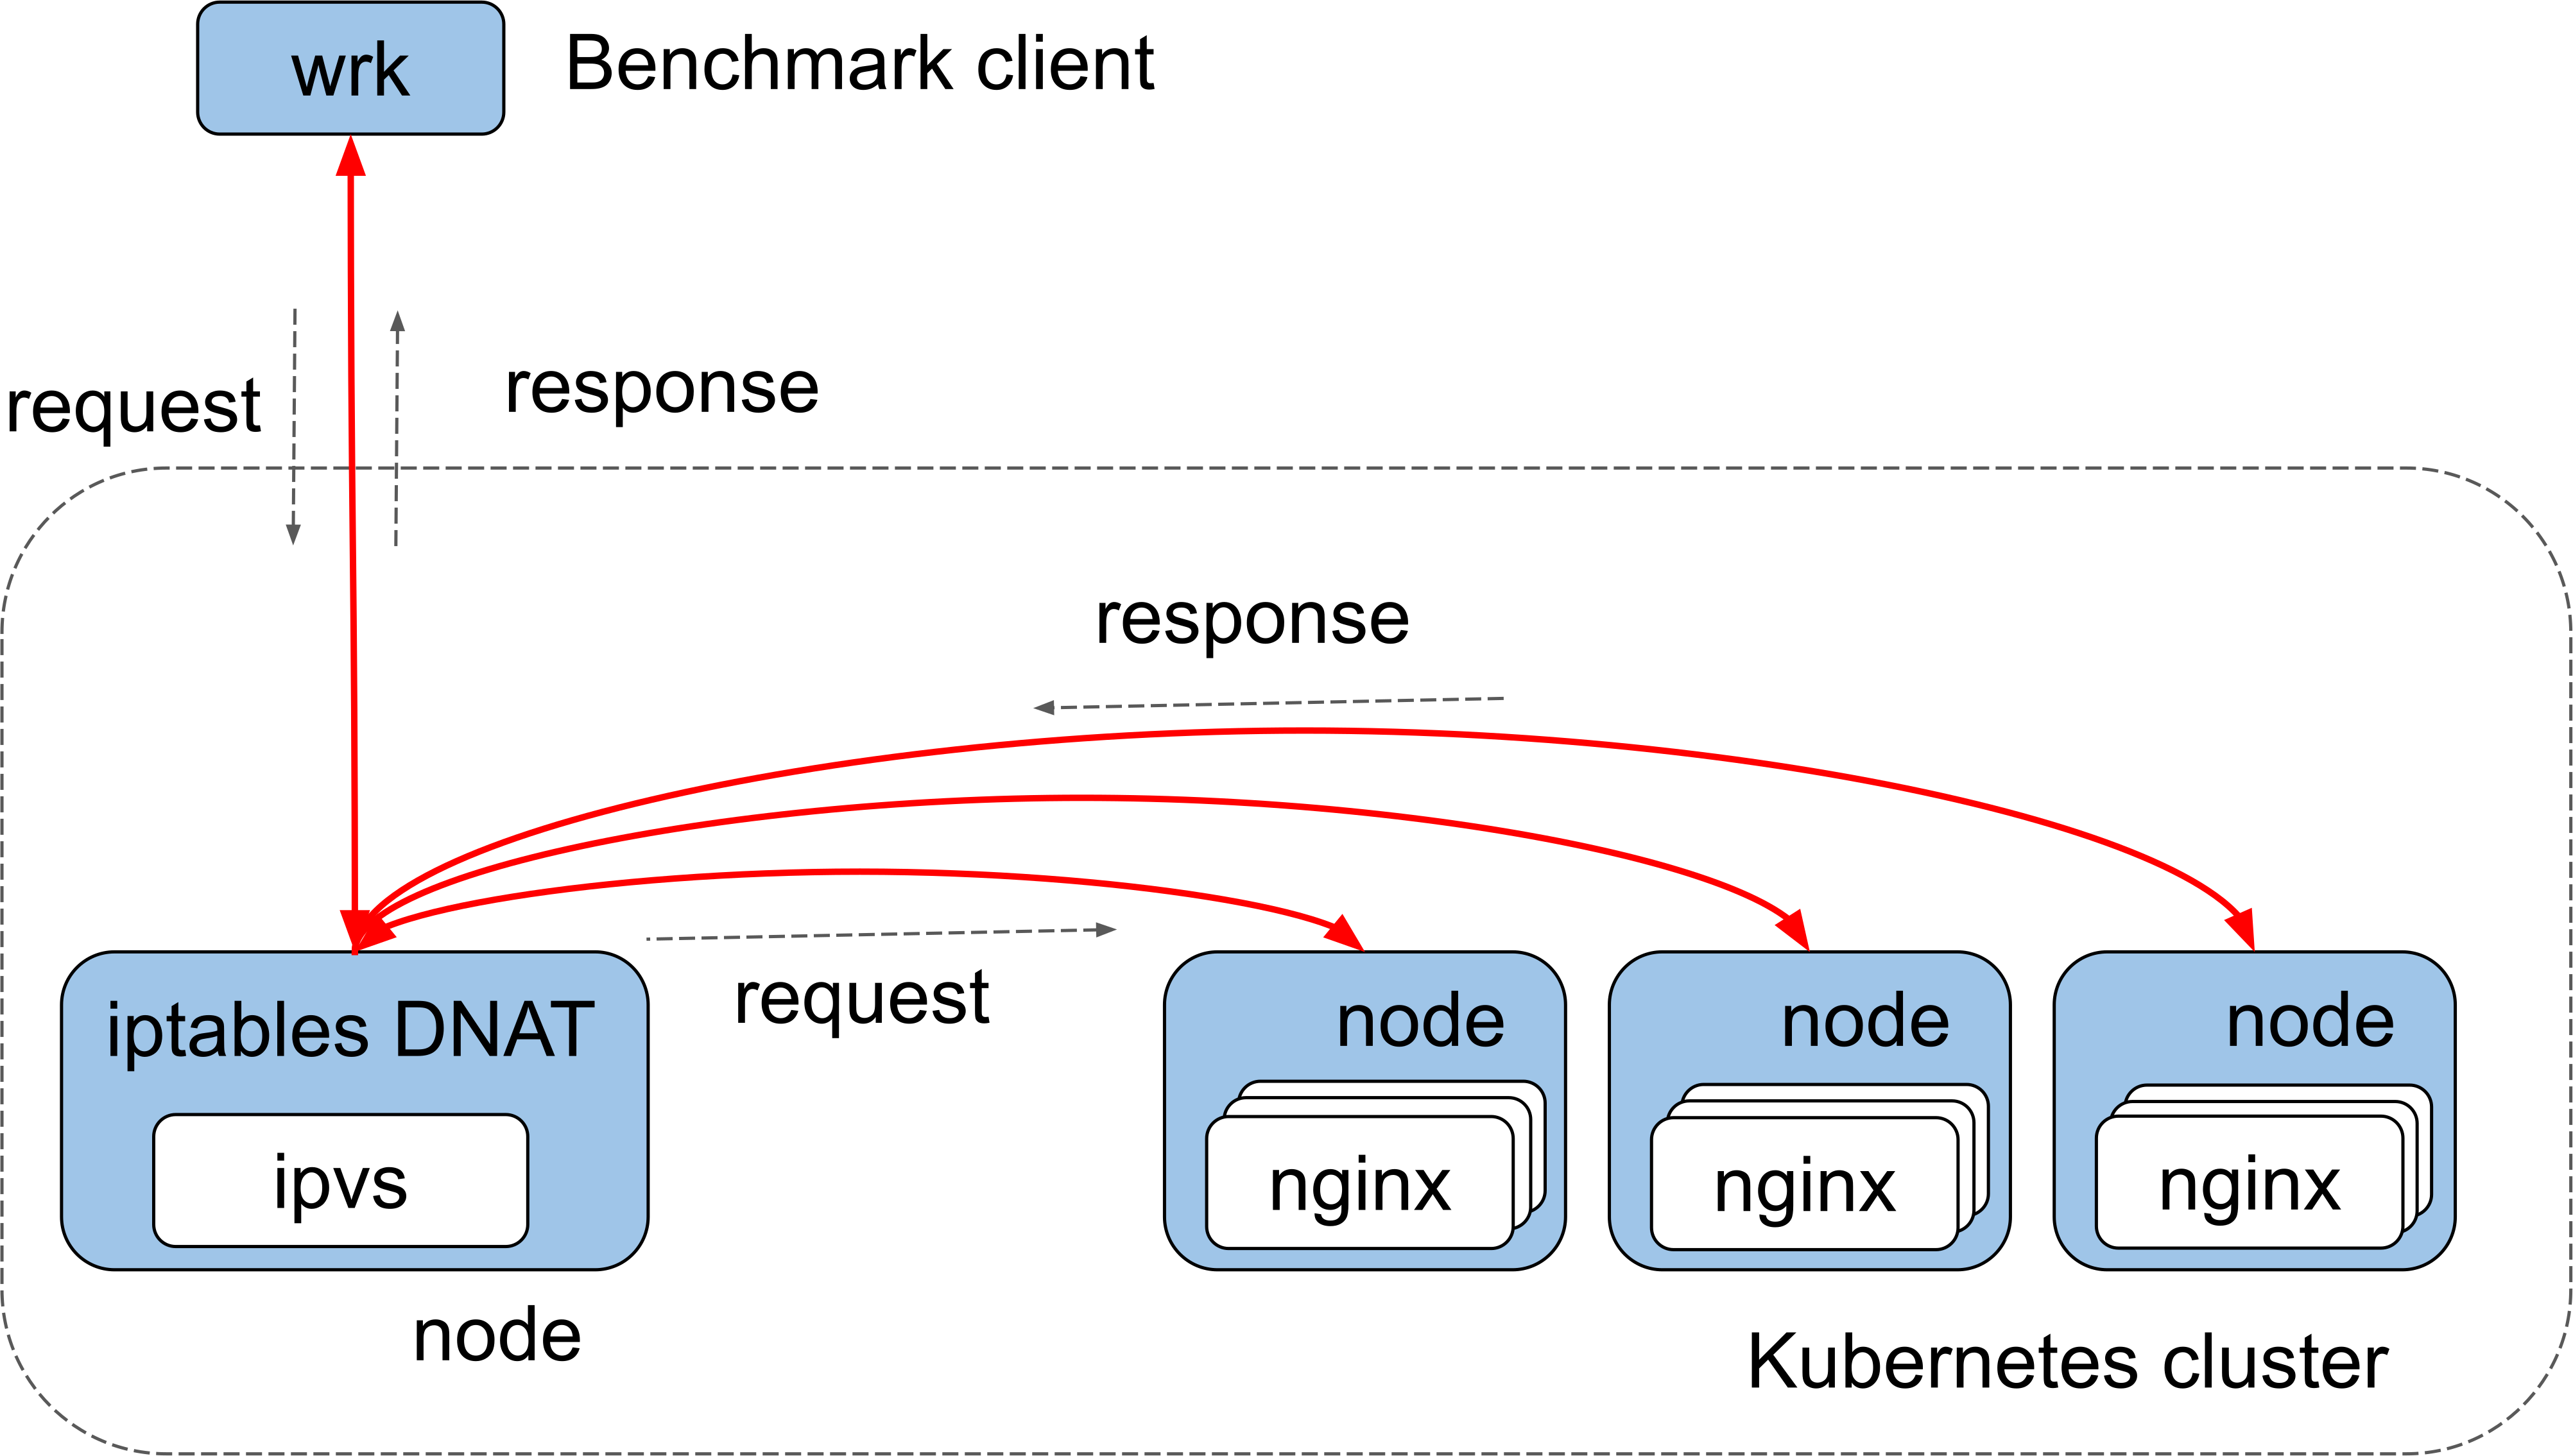
\includegraphics[width=0.8\columnwidth]{Figs/benchmark-schem-10g-nat}
    \par\bigskip
    \centering
    \begin{minipage}{0.9\columnwidth}
      \caption{}
      \label{fig:benchmark-schem-10g-nat}
    \end{minipage}
  \end{subfigure}

  \begin{subfigure}[t]{\columnwidth}
    \centering
    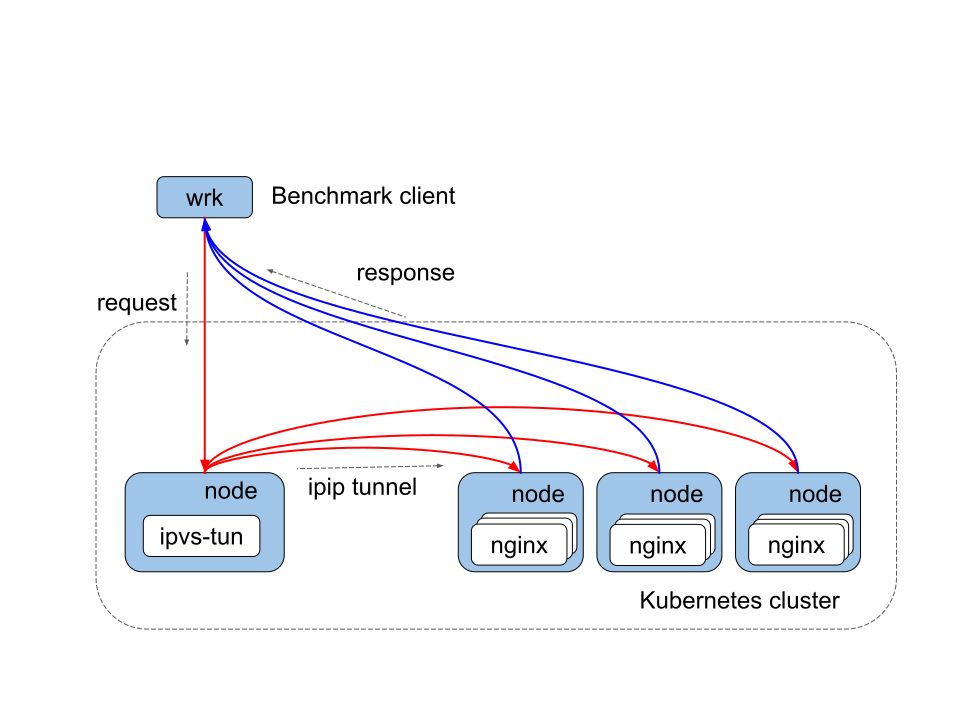
\includegraphics[width=0.8\columnwidth]{Figs/benchmark-schem-10g-dsr}
    \par\bigskip
    \centering
    \begin{minipage}{0.9\columnwidth}
      \caption{}
      \label{fig:benchmark-schem-10g-dsr}
    \end{minipage}
  \end{subfigure}

  \par\bigskip
  \centering
  \begin{minipage}{0.9\columnwidth}
    \caption[Benchmark setups in 10 Gbps experiment]{
      Benchmark setups in 10 Gbps experiment.
      (a) The setup used in throughput measurements of ipvs and iptables DNAT.
      The request and response packets both go through the load balancer node.
%      There is a bottleneck at the NIC of the load balancer node.
      (b) The setup used in throughput measurements of ipvs-tun.
      The response packets for ipvs-tun, return directly to the benchmark client.
%      The bottleneck is at the NIC of the benchmark client.
    }
    \label{fig:benchmark-schem-10g}
  \end{minipage}
\end{figure}

Figure~\ref{fig:benchmark-schem-10g} show experimental setups for the throughput measurements.
Multiple nginx {\em pods} are deployed on multiple nodes as web servers in the Kubernetes cluster.
In each nginx {\em pod}, single nginx web server program that returns the IP address of the {\em pod} itself is running.
The author then launched ipvs and ipvs-tun pod as load balancers on one of the nodes, after that, the author performed the throughput measurement changing the number of the nginx web server pods.
On every Kubernetes node, there are iptables DNAT rules that function as an internal load balancer.
The author also measured throughput of the iptables DNAT as a load balancer.
The throughput is measured by sending out HTTP requests from the wrk towards a load balancer and by counting the number of responses the benchmark client received.
In the case of the ipvs-tun, i.e., the tunneling mode of ipvs, the response packets follow the different route than the case of conventional ipvs and iptables DNAT.
As a result, the better performance level is expected for ipvs-tun since the load balancer node only has to deal with request packets of the traffic.

\FloatBarrier

Figure~\ref{fig:ipvs_l3dsr_10g} shows the throughput results of ipvs, ipvs-tun and iptables DNAT in 10Gbps environment.
The general characteristics of a load balancer, where the throughput increases linearly to a saturation level as the number of nginx container increases, can be seen.
The maximum throughput of each load balancer is limited by either packet forwarding efficiency of the software load balancer itself or the bandwidth of the network.
The maximum throughput level of the iptables DNAT is close to 780k [req/sec], where the CPU usage of the benchmark client was 100\%.
The maximum throughput levels of ipvs and ipvs-tun are less than that of iptables DNAT. 

\begin{figure}[h]
  \centering
  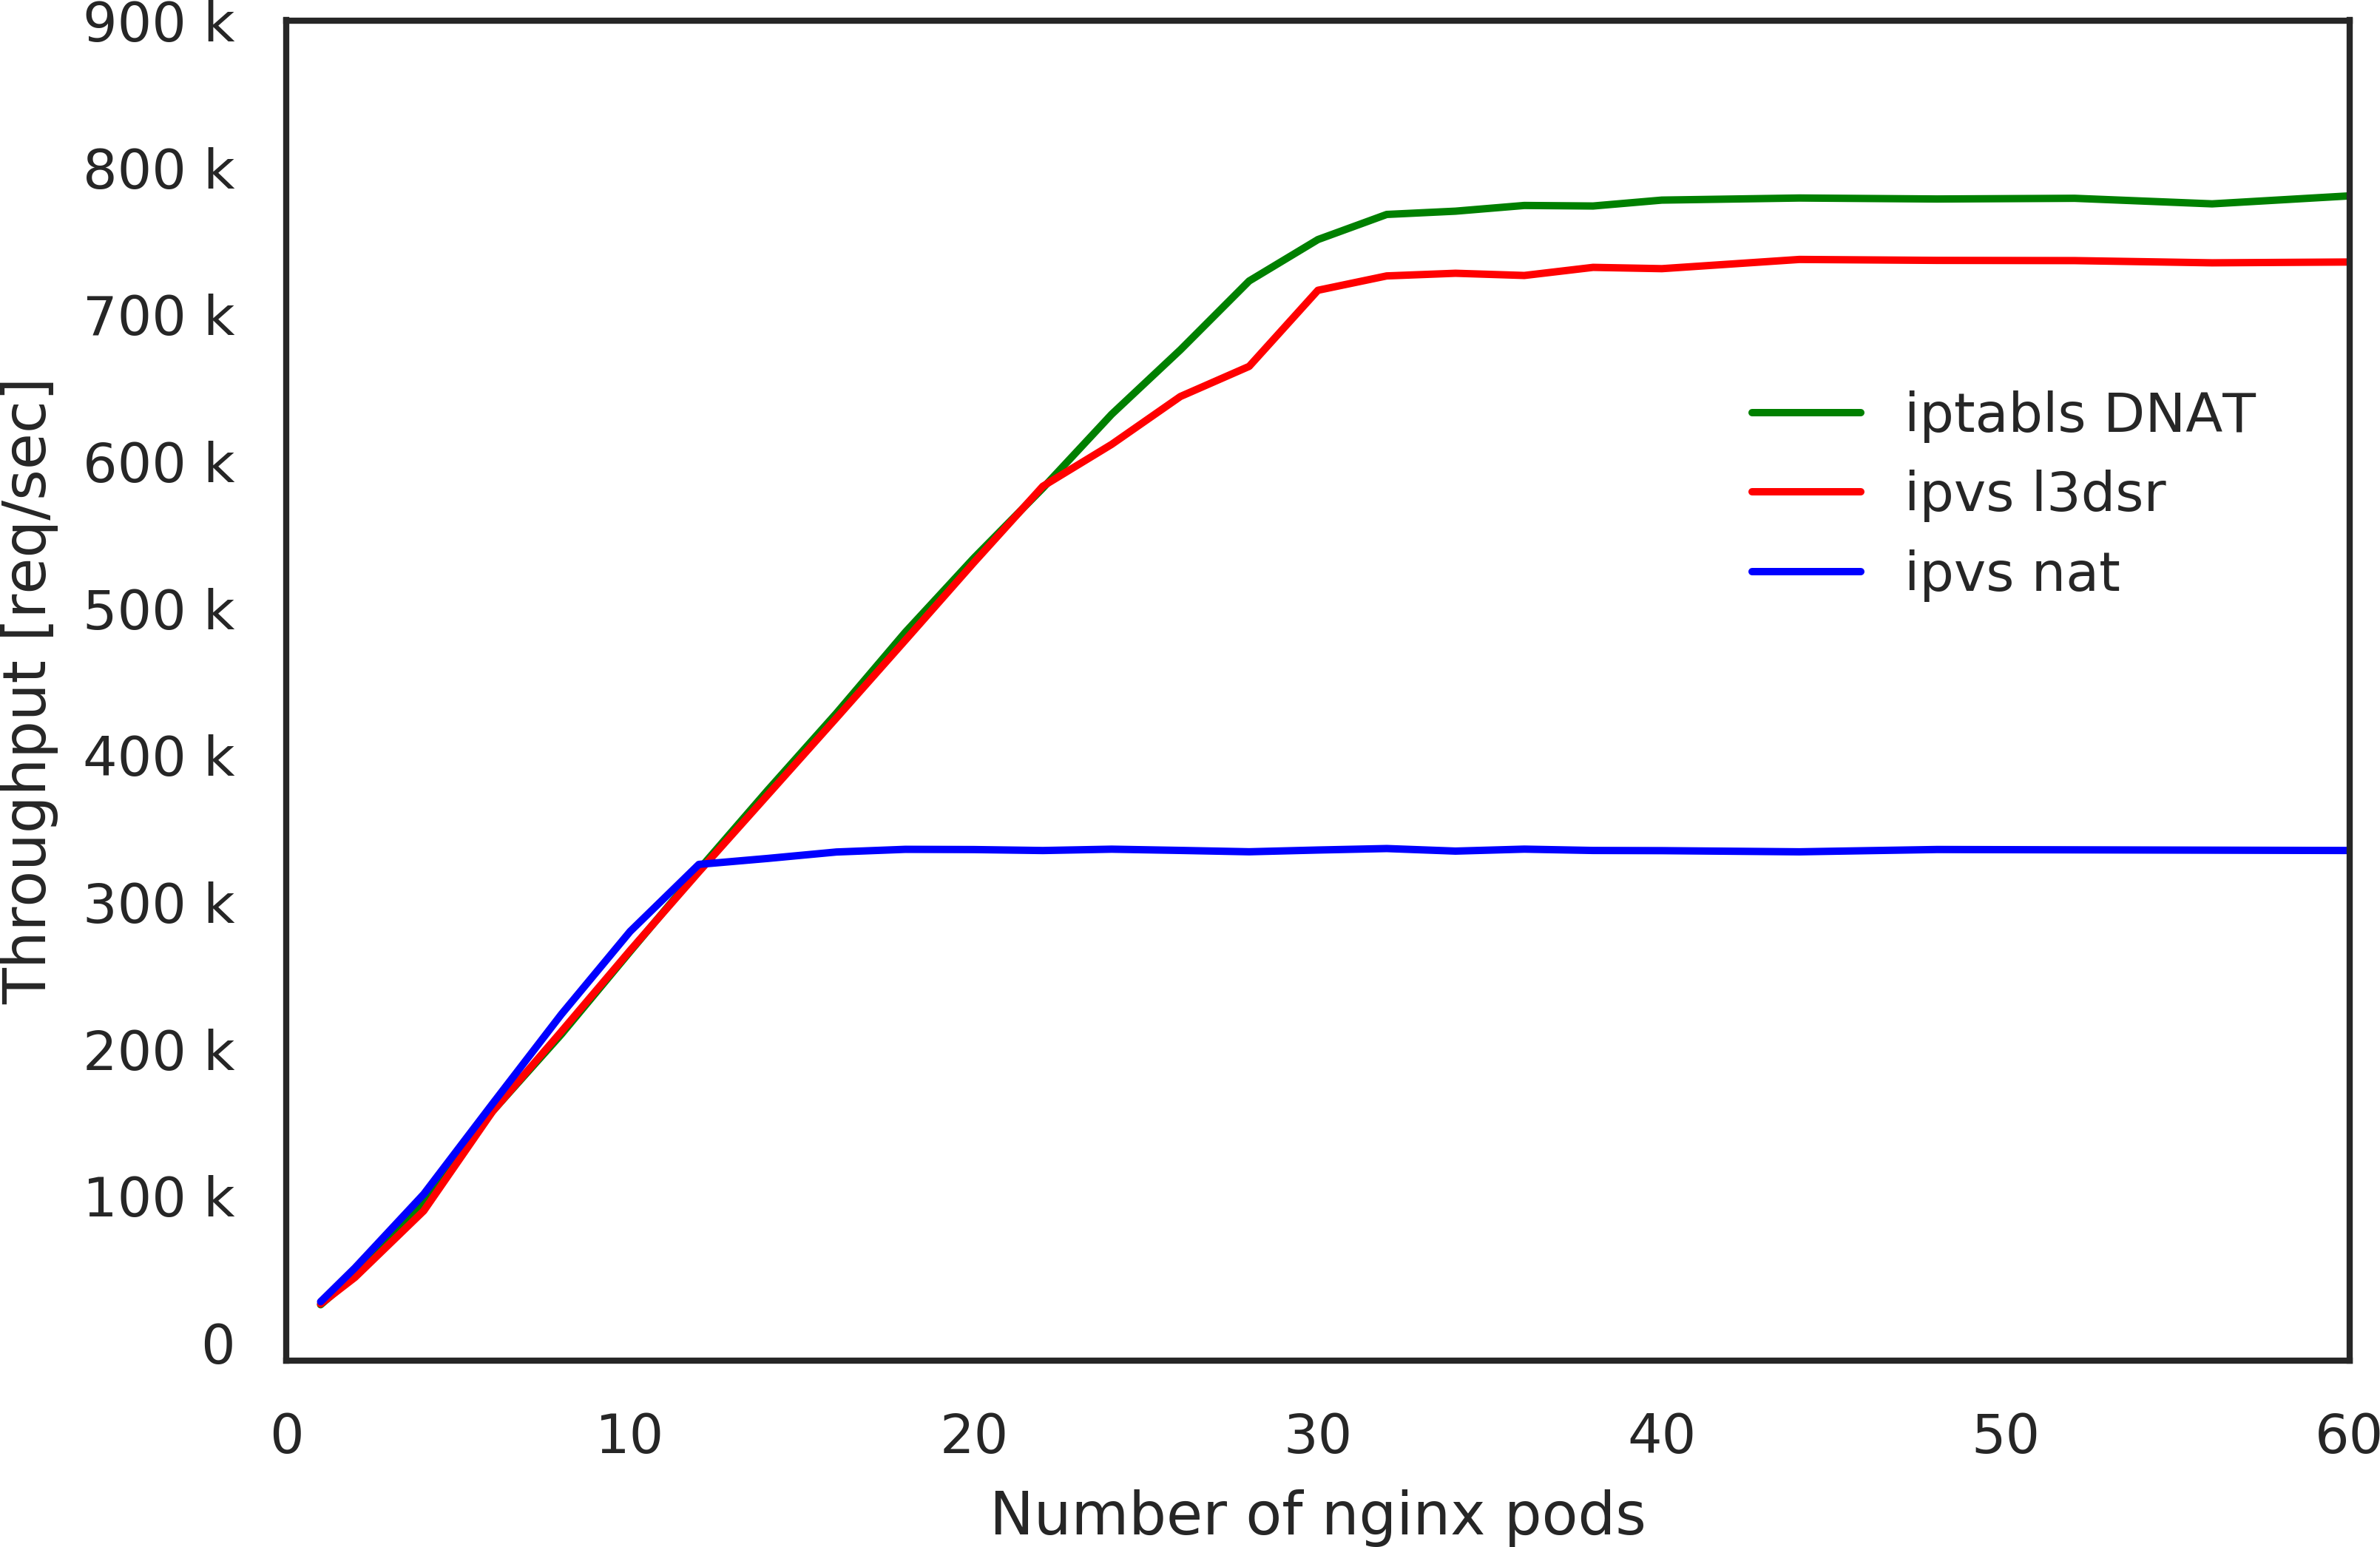
\includegraphics[width=0.8\columnwidth]{Figs/ipvs_l3dsr_10g}
  \par\bigskip
  \centering
  \begin{minipage}{0.9\columnwidth}
    \caption[Throughput of load balancers in 10 Gbps]{
      Throughput of load balancers in 10 Gbps.
      The iptables DNAT rules exist in the node net namespace.
      The ipvs and ipvs-tun are in containers.
      The throughput of the iptables DNAT is the highest.
    }
    \label{fig:ipvs_l3dsr_10g}
  \end{minipage}
\end{figure}

Figure~\ref{fig:ipvs_l3dsr_10g} shows comparison of CPU usage between load balancers.
CPU usages are sampled on the load balancer nodes at the time of the throughput measurement using a program called dstat\cite{wieers2019dstat}.
It is seen that ipvs-tun uses less CPU resource than ipvs because the load balancer node does not have to deal with the response packets.
The iptables DNAT uses even less CPU resource than ipvs and ipvs-tun.
Possible reasons for the lesser performance levels for ipvs are as follows;
(1) It is possible that the ipvs and ipvs-tun program themselves are less efficient than iptables DNAT.
(2) The network setup for the container, i.e., bridge+veth may be causing the overhead.
While iptables DNAT rules exist in node net namespace, proposed ipvs and ipvs-tun exist in container net namespace.
In order to clarify which of these is the true reason for the performance difference, the author carried out throughput measurement for ipvs and ipvs-tun without using the container network, i.e., in node net namespaces.

\begin{figure}[h]
  \centering
  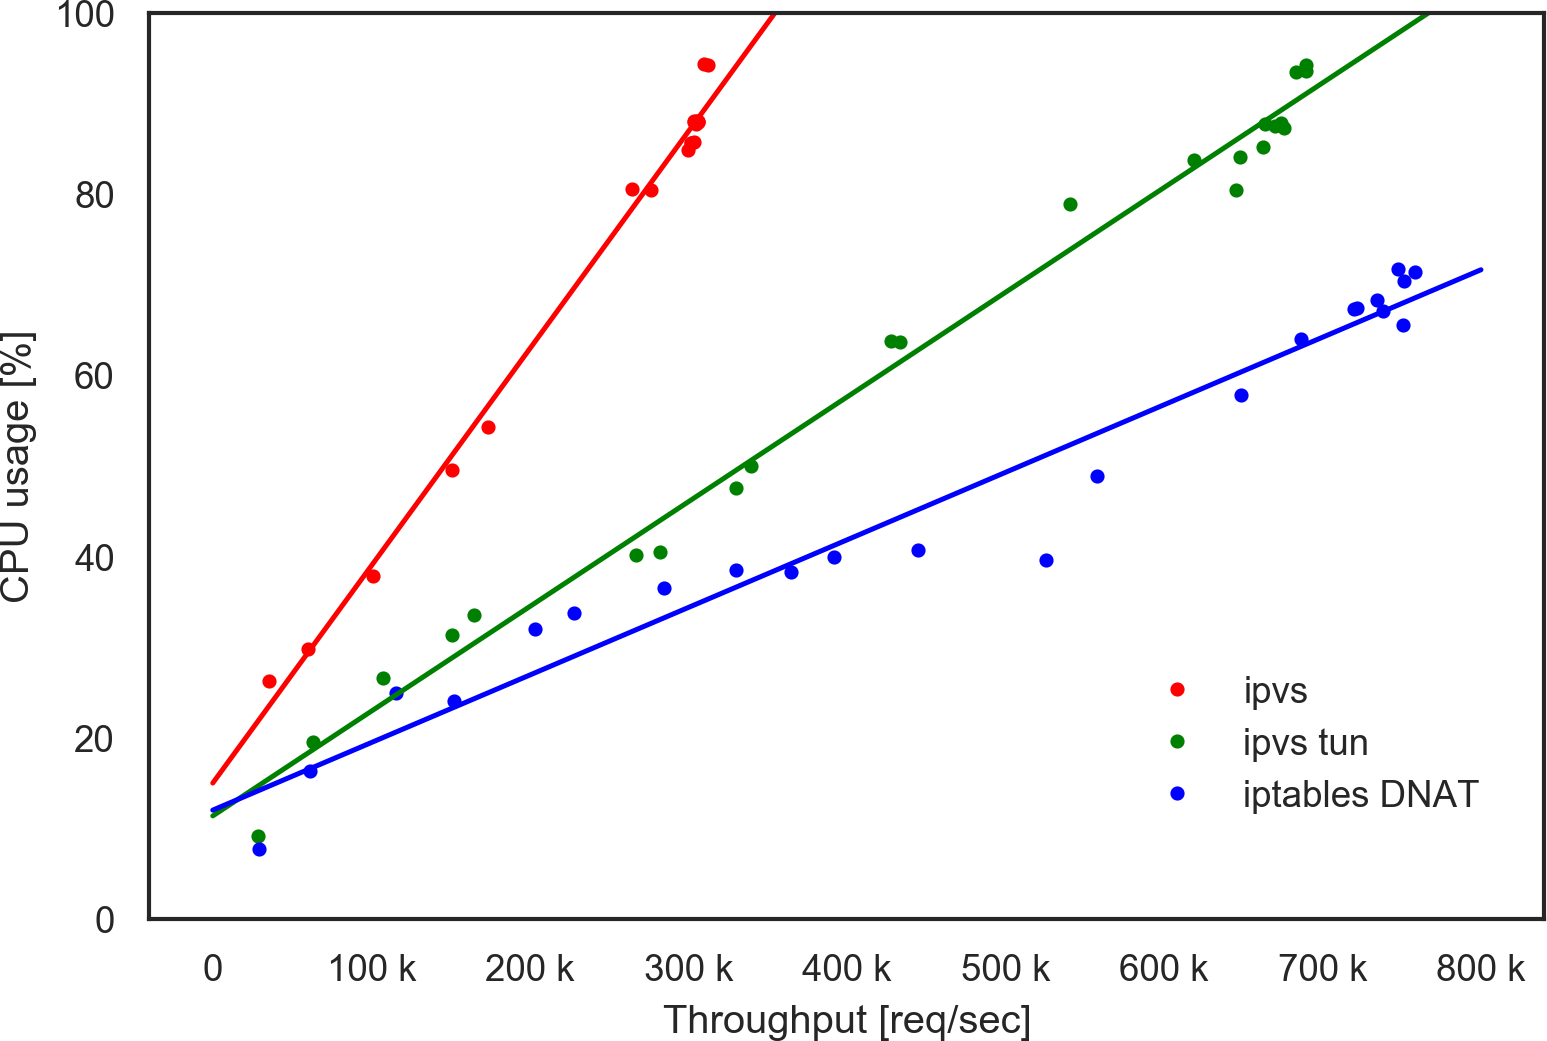
\includegraphics[width=0.8\columnwidth]{Figs/cpu_usage_10g}
  \par\bigskip
  \centering
  \begin{minipage}{0.9\columnwidth}
    \caption[CPU usage of load balancers in containers]{
      CPU usage of load balancers in containers.
      The iptables DNAT rules exist in the node net namespace.
      The ipvs and ipvs-tun are in containers.
      The iptables DNAT consumes the smallest amount of the CPU resource.
    }
    \label{fig:cpu_usage_10g}
  \end{minipage}
\end{figure}

\FloatBarrier

\subsubsection{Performance comparison in node net namespace}

The ipvs and ipvs-tun load balancers were setup on one of the nodes. 
The load balancing rules were created in the node namespaces, and then throughput measurement were carried out.

Figure~\ref{fig:ipvs_l3dsr_10g_node_ns} shows the throughput of ipvs and ipvs-tun in the node net namespace together with the throughput of the iptables DNAT.
The throughputs of the ipvs and ipvs-tun are improved from the previous results.
The throughput of the ipvs-tun is almost identical to that of iptables DNAT.
Since the CPU usages of the benchmark client were almost 100\% at the saturated throughput for ipvs and iptables DNAT, the actual maximum throughputs of these can be higher than this level.
On the other hand, the throughput of ipvs is still less than those of ipvs-tun and iptables DNAT.

\begin{figure}[h]
  \centering
  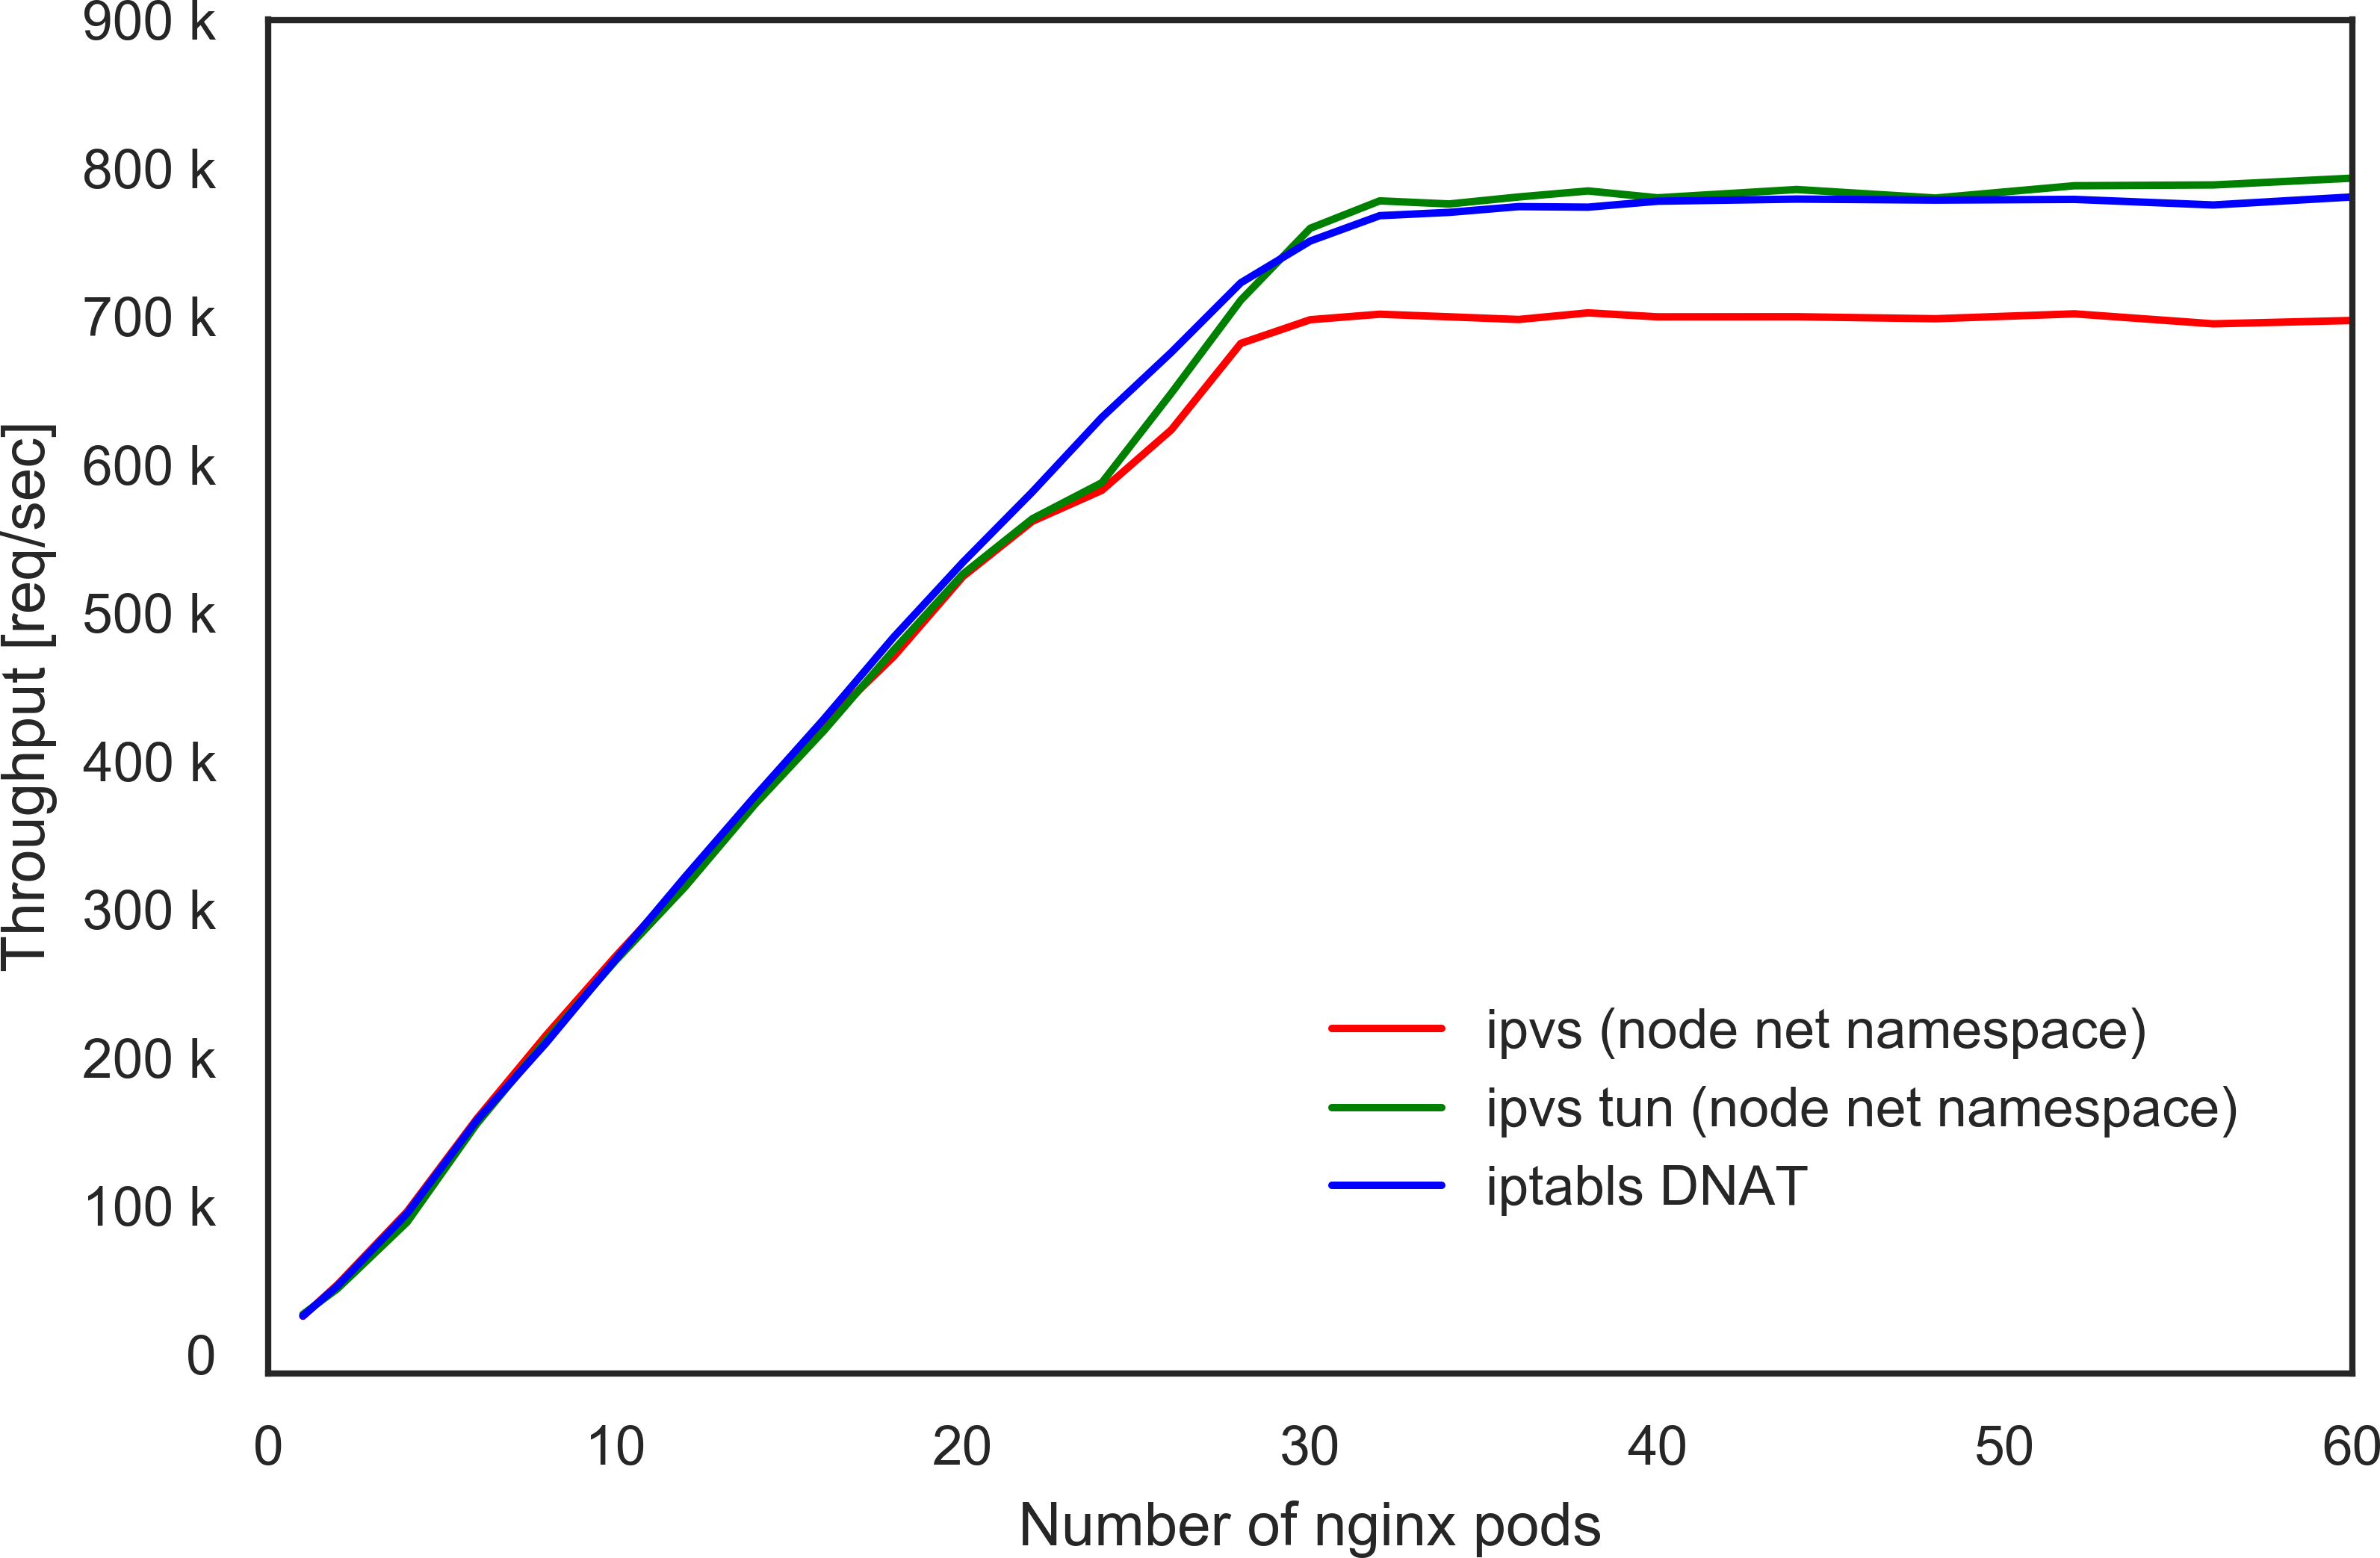
\includegraphics[width=0.8\columnwidth]{Figs/ipvs_l3dsr_10g_node_ns}
  \par\bigskip
  \centering
  \begin{minipage}{0.9\columnwidth}
    \caption[Throughput of load balancers in node namespace]{
      Throughput of load balancers in node namespace.
      The performance levels of the ipvs and ipvs-tun are greatly improved from those in Figure~\ref{fig:ipvs_l3dsr_10g} by placing them in node net namespace.
    }
    \label{fig:ipvs_l3dsr_10g_node_ns}
  \end{minipage}
\end{figure}

Figure~\ref{fig:cpu_usage_10g_node_ns} shows CPU usages of each load balancers.
While the CPU usage of the ipvs-tun becomes less than that of iptables DNAT, the CPU usage of the ipvs is still larger than that of iptables DNAT.
The author suspects that the ipvs program itself is less efficient than iptables DNAT.

\begin{figure}[h]
  \centering
  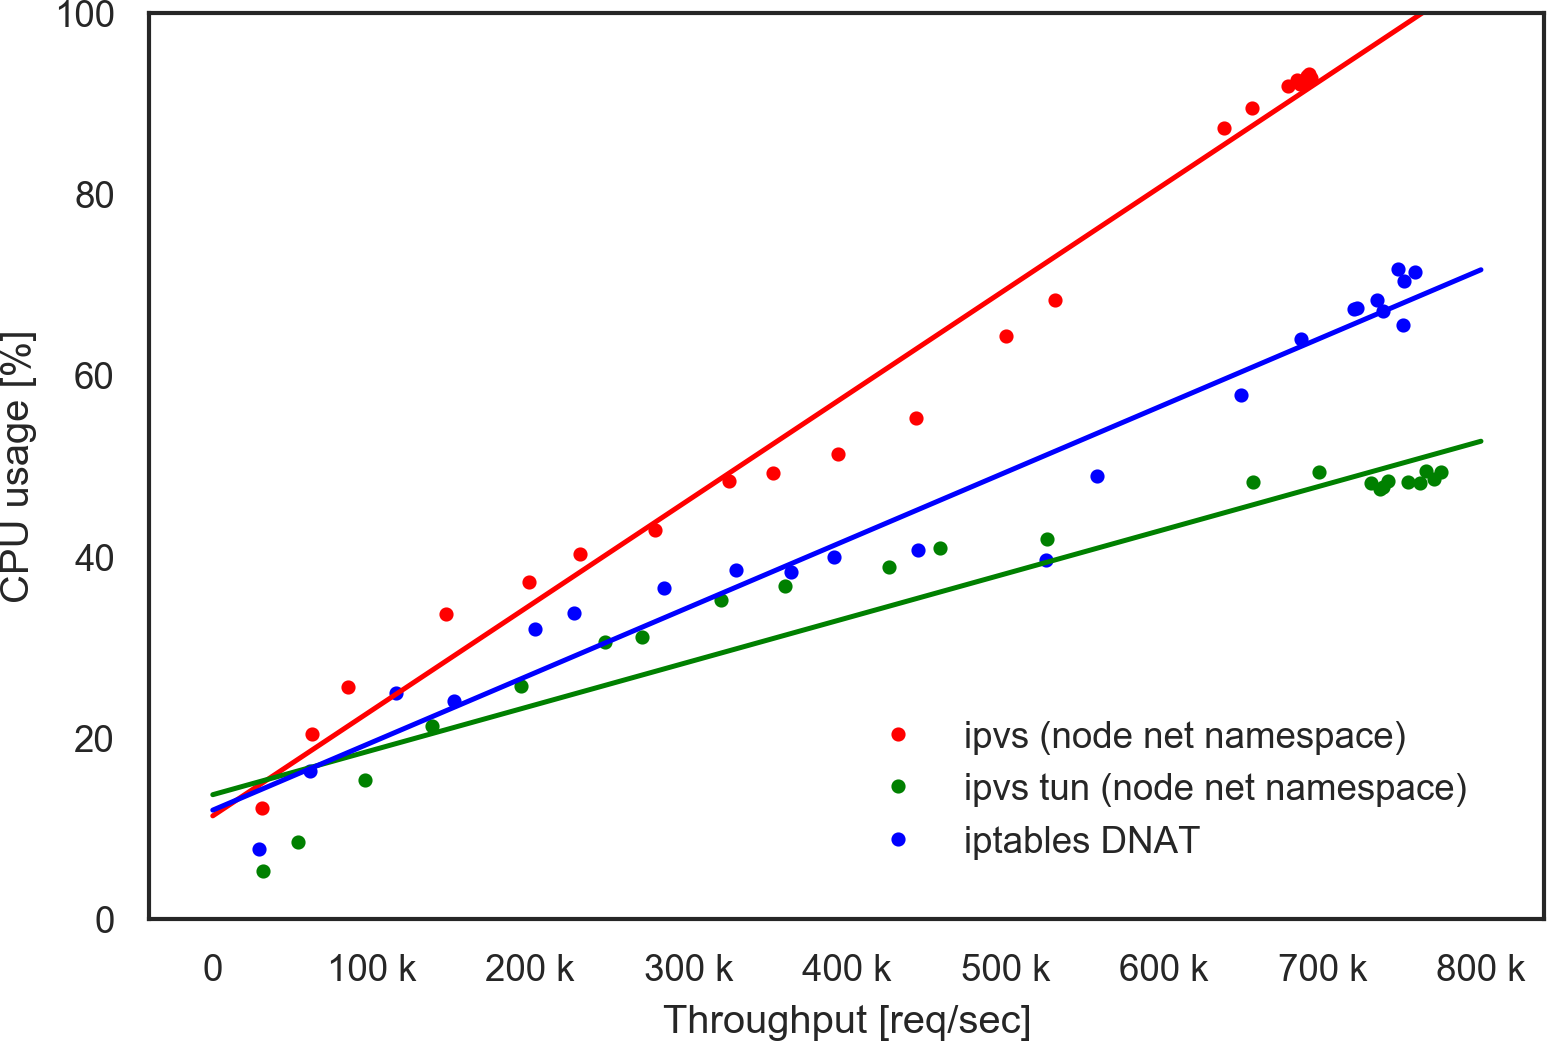
\includegraphics[width=0.8\columnwidth]{Figs/cpu_usage_10g_node_ns}
  \par\bigskip
  \centering
  \begin{minipage}{0.9\columnwidth}
    \caption[CPU usage of load balancers on nodes]{
      CPU usage of load balancers on nodes.
      CPU usages of ipvs and ipvs-tun greatly improved from those in Figure~\ref{fig:cpu_usage_10g} by placing them in node net namespace.  
      While the ipvs-tun consumes the smallest amount of the CPU resource, the CPU usage of ipvs is still larger than that of iptables DNAT.
    }
    \label{fig:cpu_usage_10g_node_ns}
  \end{minipage}
\end{figure}

The author summarizes this section as follows;
The ipvs itself is less efficient than iptables DNAT.
Using the container network, i.e., veth+bridge further degrades the throughput of ipvs.

\FloatBarrier

\section{Discussion of required throughput}

The author has compared the performance of proposed load balancers in 10Gbps in the previous section.
Although the proposed load balancer may not be the most efficient one, it is still useful because of the lateral scalability.

Table~\ref{tab:performance_summary} summarizes the maximum throughputs of the different load balancers obtained in the experiments so far.
Depending on the experimental conditions different part of the setup limits the throughput of the load balancers.
Since the performance bottlenecks are mainly due to network bandwidth in 1Gbps network, it is easy to estimate the possible bottleneck due to bandwidth in a faster network.
Since benchmark client exists at the location where normally the upstream router exists, the performance bottleneck at the benchmark client corresponds to the maximum throughput that the load balancer should handle..

For example, the bottleneck at the benchmark client is about 293K [req/sec] in the 1Gbps network. 
The load balancers only need to be able to handle at most 293K [req/sec] equivalent traffic.
Even if the load balacer is capable of handling 500K [req/sec], the throughput of the system is ultimately determined by the bottleneck at the entrance, that is 293K [req/sec].
The maximum throughput in 1Gbps, i.e., 293K [req/seq] is easily achieved by single ipvs-tun (293K [req/seq]) or two of ipvs load balancers (193K x 2 [req/seq]) with ECMP redundancy.

In the case of 10Gbps network, the maximum throughput determined by the bottleneck at the entrance is 2.9M [req/sec].
This is still easily achievable by using four of ipvs-tun (731K x 4 [req/seq]) or nine of ipvs load balancers (335K x 9 [req/seq]) with ECMP redundancy.

In the case of 100Gbps network, where the load balancers are required to accommodate up to throughput of 29M [req/sec], the inefficiency of the software load balancer in a container can become a real problem.
Because in order to handle 29M [req/sec] of the traffic, 90 of ipvs load balancer will be needed.
In the next section, the author tries to improve the efficiency of a load balancer, by implementing novel XDP load balancer.

\begin{table}[h]

  \begin{subtable}{1\textwidth}
    \centering
    \begin{tabular}{|l|l|c|l|}
      \hline
      \multicolumn{1}{|c|}{Type} & \multicolumn{1}{c|}{namespace} &
      \begin{tabular}{c} Throughput \\ {[}req/sec{]} \end{tabular} & \multicolumn{1}{c|}{Bottleneck} \\ \hline
      iptables DNAT & node      & 193K &
      \begin{tabular}{l} Bandwidth filled with request \\ + response @ load balancer \end{tabular} \\ \hline
      ipvs          & container & 197K &
      \begin{tabular}{l} Bandwidth filled with request \\ + response @ load balancer \end{tabular} \\ \hline
      ipvs-tun      & container & 293K &
      \begin{tabular}{l} Bandwidth filled with response \\ @ benchmark client  \end{tabular} \\ \hline
    \end{tabular}
    \caption{1Gbps experiment}
  \end{subtable}

  \par\bigskip

  \begin{subtable}{1\textwidth}
    \centering
    \begin{tabular}{|l|l|c|l|}
      \hline
      \multicolumn{1}{|c|}{Type} & \multicolumn{1}{c|}{namespace} &
      \begin{tabular}{c} Throughput \\ {[}req/sec{]} \end{tabular} & \multicolumn{1}{c|}{Bottleneck} \\ \hline
      iptables DNAT & node      & 778K & \begin{tabular}{l} CPU\(\sim\)100\% @ benchmark client\end{tabular} \\ \hline
      ipvs          & container & 335K & \begin{tabular}{l} CPU\(\sim\)100\% @ load balancer node\end{tabular} \\ \hline
        ipvs-tun      & container & 731K & \begin{tabular}{l} CPU\(\sim\)100\% @ load balancer node\end{tabular} \\ \hline
          ipvs          & node      & 700K & \begin{tabular}{l} CPU\(\sim\)100\% @ load balancer node\end{tabular} \\ \hline
      ipvs-tun      & node      & 780K & \begin{tabular}{l} CPU\(\sim\)100\% @ benchmark client\end{tabular} \\ \hline
   \end{tabular}
      \caption{10Gbps experiment}
  \end{subtable}

  \par\bigskip
  \centering
  \begin{minipage}{0.9\columnwidth}
    \caption[Summary of the maximum throughputs]{
      Summary of the maximum throughputs.
    }
    \label{tab:performance_summary}
  \end{minipage}
\end{table}

\FloatBarrier

\section{XDP load balancer}

The eXpress Data Path(XDP) is Linux kernel technology recently developed, where the tools and functionality to incept and process the packets in the earlist phase as possible are provided.
By utilizing XDP, one can hook a byte-compiled code developed in subset of the C programing language, to a place before the socket buffer is assigned, thereby speeding up network manupulation, including block against DDOS atack, simple packet forwarding and load balancing.
The one of the benefit of the XDP compared to DPDK is that in the case XDP, the packtes that do not match the rule for processing are then passd to normal Linux network stack.
Therefore there is no need for preparing dedicated NIC for fast and efficient network processing.
The author implemented the XDP load balacer and carried out throughput measurement.

\subsubsection{Implementation}

\subsubsection{Benchmark setup}

\subsubsection{Throughput results }

The author carried out the throughput measurement for the XDP load balacer, xlb.
The hardware and software configuretions are same as the ones in Table~\ref{tab:hw_sw_spec_10g}.
The exprimental setup is also same as the one in Figure~\ref{fig:benchmark-schem-10g}(b).
Since current implementation of xlb does not support multi core packet processing, the setting \enquote{(RSS,RPS)=(off,off)} is used in the throughput measurement.
All the intterrupt from the NIC are notified to a single core.

Figure~\ref{fig:cpu_usage_10g_xlb} compares the throughput of xlb and iptables DNAT. 
Although a single core is used for the packet processing, the throughput of the xlb load balancer is close to half of the iptables DNAT's throughput with 16 core(eight physical cores) packet processing.
Figure\ref{fig:cpu_usage_10g_xlb} compares CPU usages between xlb and iptables DNAT.
At a given throughput the xlb consumes much less CPU resource than iptables DNAT.
These results indicate that load balancer using XDP technology is very promising.

\begin{figure}[h]
  \centering
  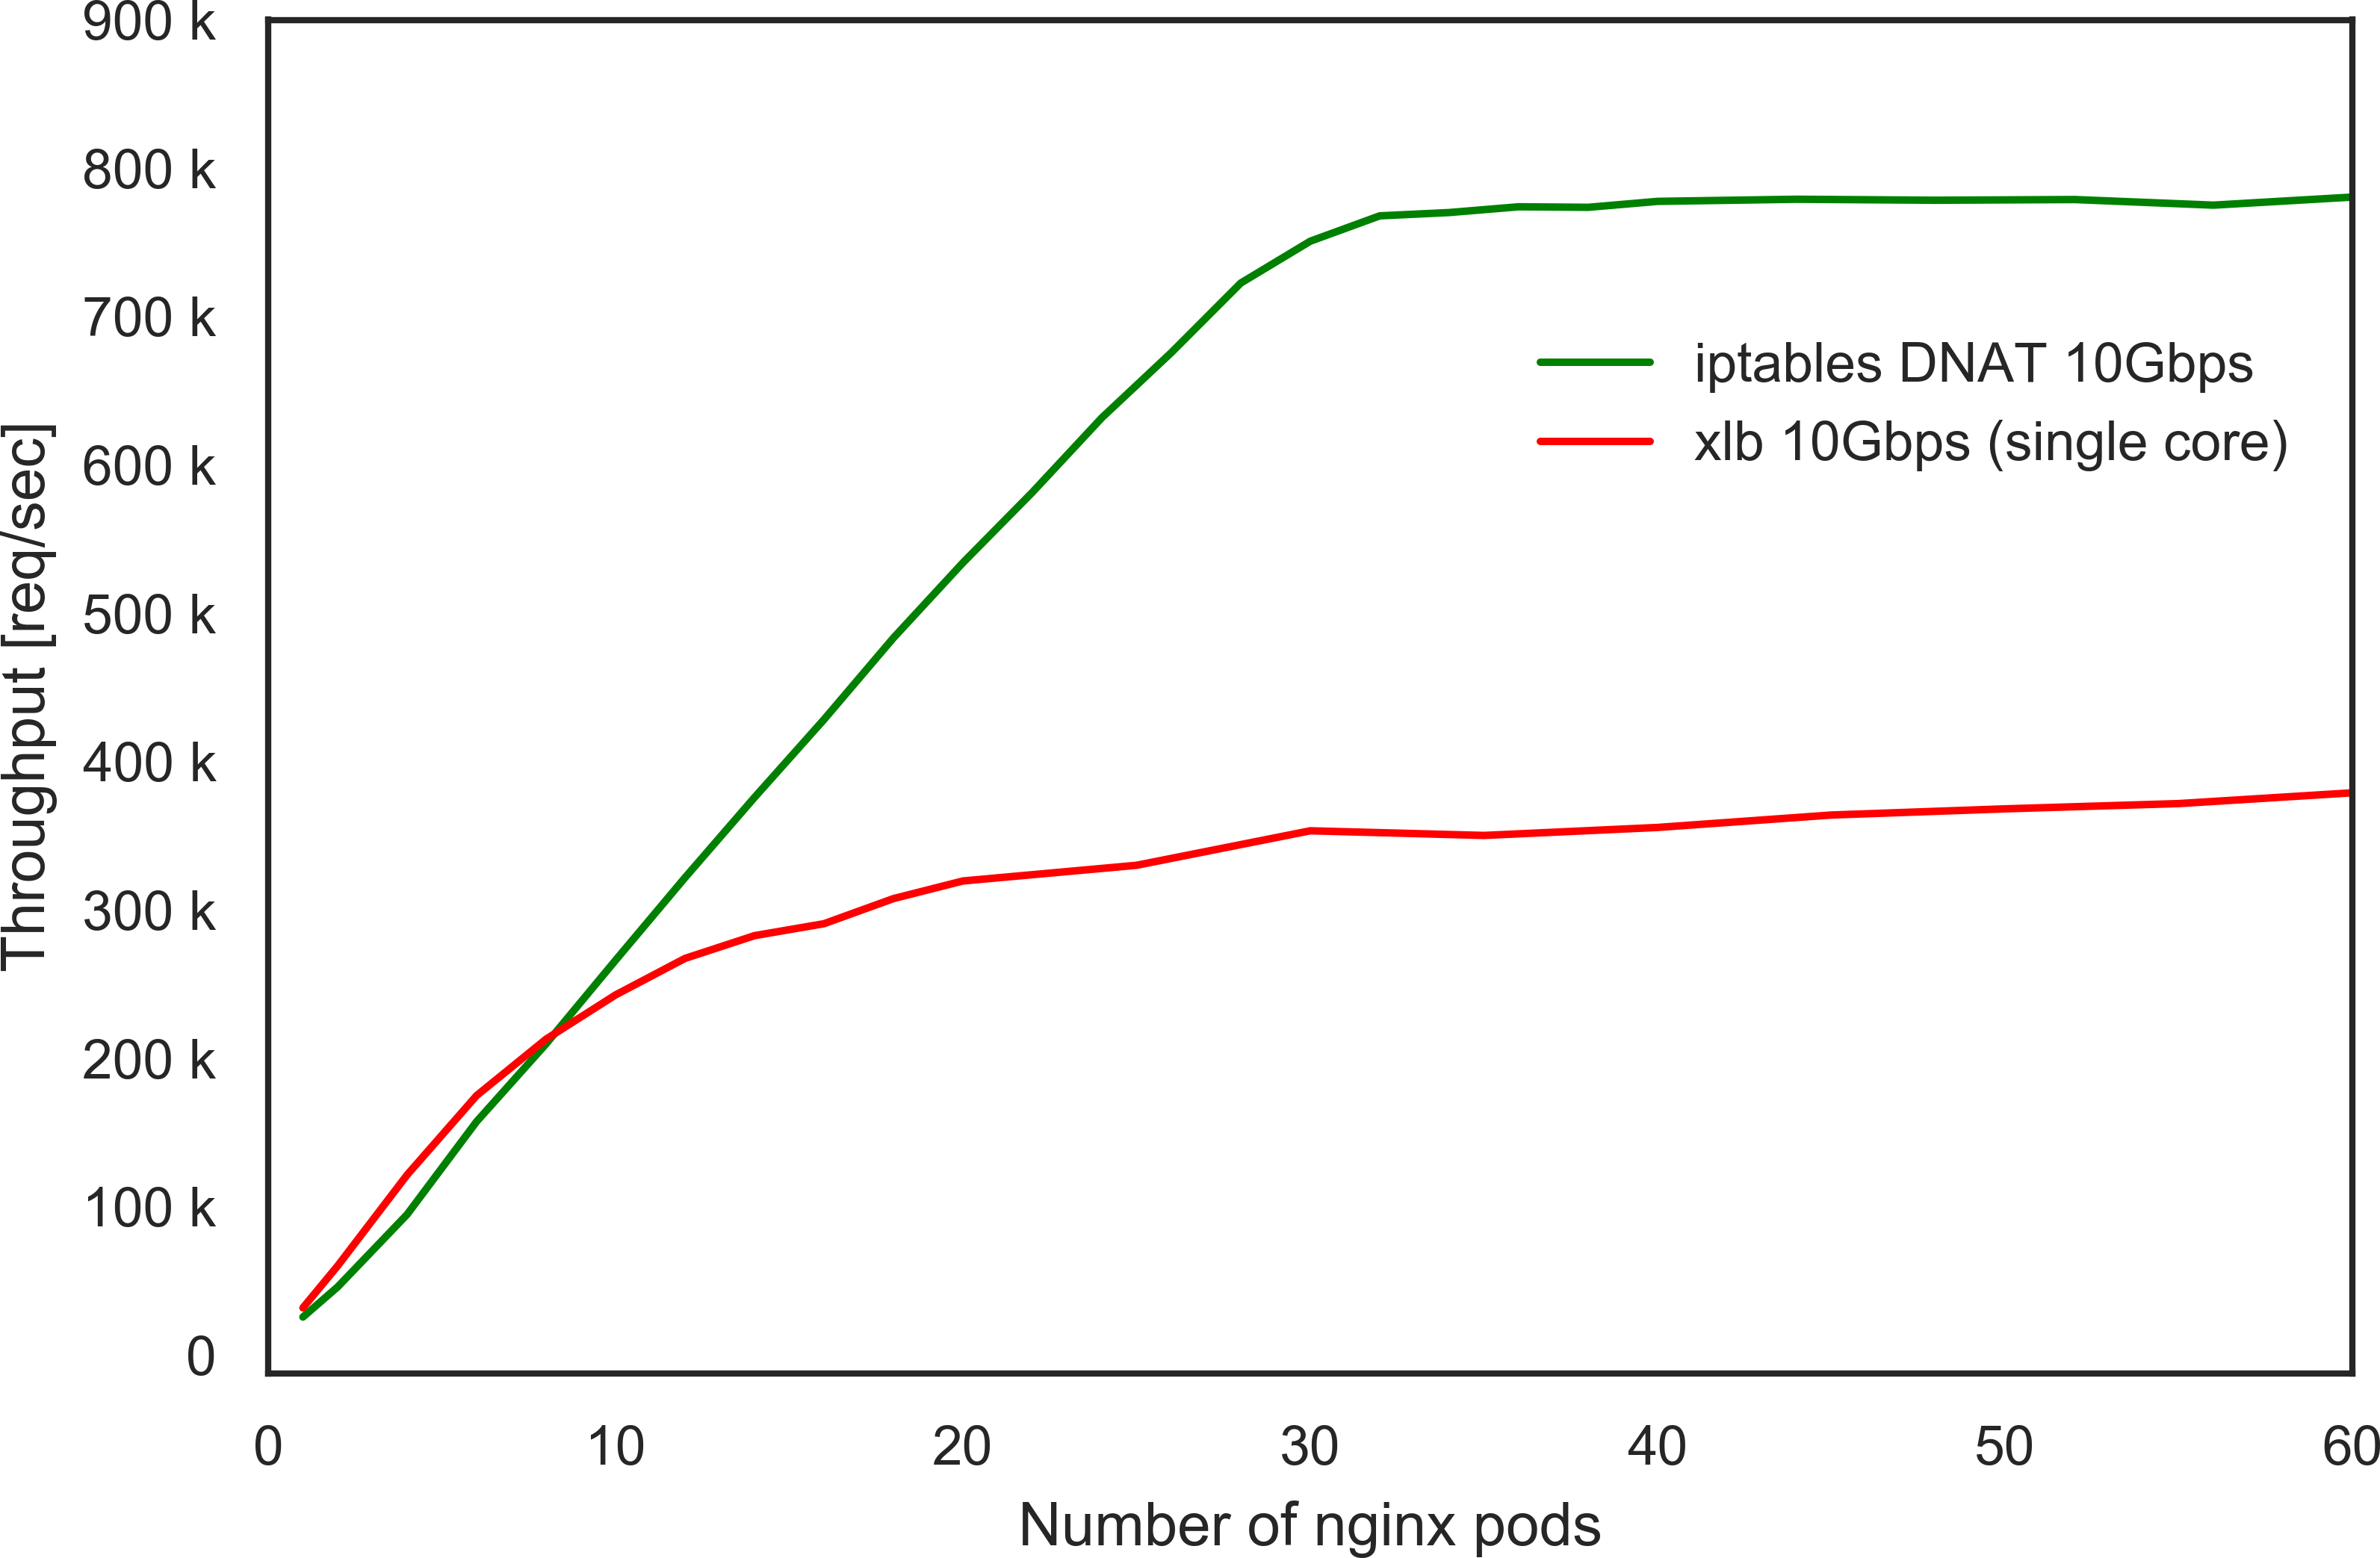
\includegraphics[width=0.8\columnwidth]{Figs/xlb_iptables_dnat_10g}
  \par\bigskip
  \centering
  \begin{minipage}{0.9\columnwidth}
    \caption[Throughput of xlb load balancer]{
      Throughput of xlb load balancer.
      The xlb load balancer is placed in node net namespace.
      The setting \enquote{(RSS,RPS)=(off,off)}, i.e., single core packet processing is used for the xlb measurement.
      The results of iptables DNAT for \enquote{(RSS,RPS)=(on,off)} and \enquote{(RSS,RPS)=(off,off)} are also shown for comparison.
      The throughput of the xlb is much higher than that of iptables DNAT with single core packet processing.
      Although using only a single core for, the throughput of the xlb load balancer is close to half of the iptables DNAT's with 16 core(eight physical corex) pakcet processing.
    }
    \label{fig:xlb_iptables_dnat_10g}
  \end{minipage}
\end{figure}


\begin{figure}[h]
  \centering
  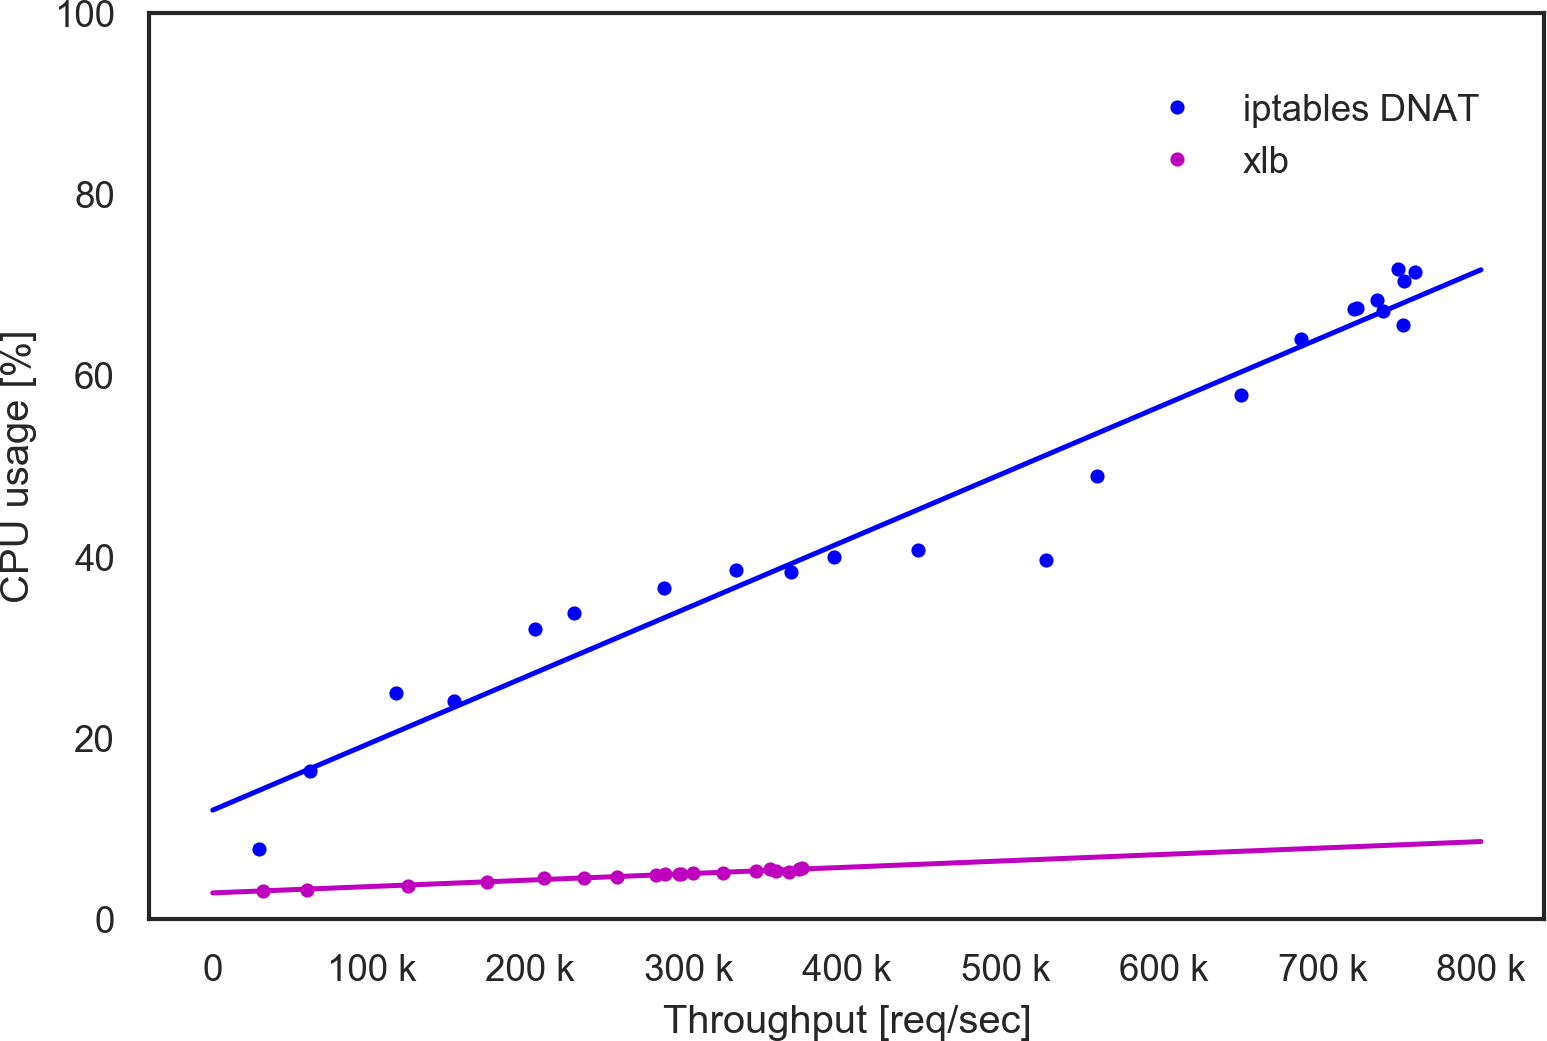
\includegraphics[width=0.8\columnwidth]{Figs/cpu_usage_10g_xlb}
  \par\bigskip
  \centering
  \begin{minipage}{0.9\columnwidth}
    \caption[CPU usage of xlb load balancer]{
      CPU usage of xlb load balancer.
      The xlb uses much less CPU resource than iptables DNAT.
    }
    \label{fig:cpu_usage_10g_xlb}
  \end{minipage}
\end{figure}

\FloatBarrier

\section{Summary}

In this chapter, the author carried out throughput measurements of ipvs, ipvs-tun, and iptables DNAT in 10Gbps environment.
From the results, the general characteristics of a load balancer are observesd.
The throughputs of ipvst and ipvs-tun are smaller than that of iptables DNAT in 10Gbps network, both due to the overhead of the container network and inefficiency in the program itself.
In order to improve the performance levels of portable load balancer, better network setup for containers and more efficient load balancer software should be developed.

However, considering the fact that the ultimate throughput of the system does not exceed that of the upstream router, the entrance, 
the load balancers only need to be able to handle at most 293K, 2.9M, and 29M [req/sec], in 1Gbps, 10Gbps, and 100Gbps, respectively.
Since a single ipvs in container can handle 335K [req/sec], traffic equivalent to 2.9M [req/sec], which is the maximum throughput achievable in 10Gbps, can be easily handled by nine of ipvs containers.

The author also presented the priliminary result of xlb experiment, which will be needed in 100Gbps network environment.
The obtained per core throughput result and CPU usage result have been very promising.

